% Homework Specific Commands
\newcommand{\CMX}{\text{CMX}}
\newcommand{\ORD}{\text{ORD}}
\newcommand{\DTW}{\text{DTW}}
\newcommand{\MQT}{\text{MQT}}
\newcommand{\MSP}{\text{MSP}}


\begin{document}
\extrawidth{0.5in} \extrafootheight{-0in} \pagestyle{headandfoot}
\headrule \header{\textbf{CS2311 - Spring 2021}}{\textbf{HW
 5  \ifprintanswers - Solutions \fi}}{\textbf{Due: ***. **/**/21}} \footrule \footer{}{Page \thepage\
of \numpages}{}

\ifprintanswers
\noindent \textbf{Instructions:} All assignments are due \underline{by
\textbf{midnight} on the due date} specified.  Assignments should be typed or
scanned and submitted as a PDF in Canvas.

\medskip
\noindent Every student or student group must write up their own solutions in
their own manner.

\medskip
\noindent You should \underline{complete all problems}, but \underline{only a
subset will be graded} (which will be graded is not known to you ahead of
time).
\else
\noindent \textbf{Instructions:} All assignments are due \underline{by \textbf{midnight} on the due date} specified.

\medskip
\noindent Every student or student group  must write up their own solutions in
their own manner.

\medskip
\noindent Please present your solutions in a clean, understandable
manner.  Use the provided files that give mathematical notation in Word, Open Office, Google Docs, and \LaTeX.

\medskip
\noindent Assignments should be typed or scanned and submitted as a PDF.

\medskip
\noindent You should \underline{complete all problems}, but \underline{only a
subset will be graded} (which will be graded is not known to you ahead of
time).
\fi

\begin{questions}



\section*{Graphs}

\gquestion{2}{2}{all} Rosen Ch 10.2.56, p. 702.
    \ifprintanswers
        \vspace{-12pt}
    \fi
    \begin{solution}
        The graphs $K_{m,n}$ are regular if and only if $m=n$.
    \end{solution}



\gquestion{3}{3}{all} Rosen Ch 10.3.40, p. 711. 
    \ifprintanswers
        \vspace{-10pt}
    \fi
    \begin{solution}
    First check the invariants.  Graph $U$ and $V$ both have 5 vertices. Graph $U$ and $V$ both have 7 edges.

    Graph $U$ has 1 vertex of degree 2 and 4 vertices of degree 3.  Graph $V$ has 2 vertices of degree 2, 2 vertices of degree 3 and one vertex of degree 4. 

    The graphs are \textbf{not isomorphic}.
    \end{solution}



\ugquestion{3} Rosen Ch 10.3.42, p. 712.
    \ifprintanswers
        \vspace{-10pt}
    \fi
    \begin{solution}
    First check the invariants.  Graph $U$ and $V$ both have 5 vertices. Graph $U$ and $V$ both have 8 edges. Graph $U$ has 1 vertex with degree=2, 2 vertices with degree=3, and 2 vertices with degree=4.  Graph $V$ has 1 vertex with degree=2, 2 vertices with degree=3, and 2 vertices with degree=4.  Several possible  isomorphisms are listed below.
    
            $ f(u_1) = v_1, f(u_2) = v_3, f(u_3) = v_2, f(u_4) = v_5, f(u_5) = v_4 $\\
            $ f(u_1) = v_4, f(u_2) = v_5, f(u_3) = v_2, f(u_4) = v_3, f(u_5) = v_1 $ \\
            $ f(u_1) = v_1, f(u_2) = v_5, f(u_3) = v_2, f(u_4) = v_3, f(u_5) = v_4 $\\
            $ f(u_1) = v_4, f(u_2) = v_3, f(u_3) = v_2, f(u_4) = v_5, f(u_5) = v_1 $
    \end{solution}


% \gquestion{3} Rosen Ch 10.3 \# 40, p. 676.
%    \ifprintanswers
%         \vspace{-10pt}
%    \fi
%     \begin{solution}
%     First check the invariants. Graph $U$ and $V$ both have 6 vertices.  Graph $U$ and $V$ both have 8 edges.  Graph $U$ has 2 vertices with degree=2 and 4 vertices with degree=3.  Graph $V$ has 3 vertices with degree=2, 2 vertices with degree=3, and 1 vertex with degree=4.  The graphs are \textbf{not isomorphic}.
%     \end{solution}



\begin{center}
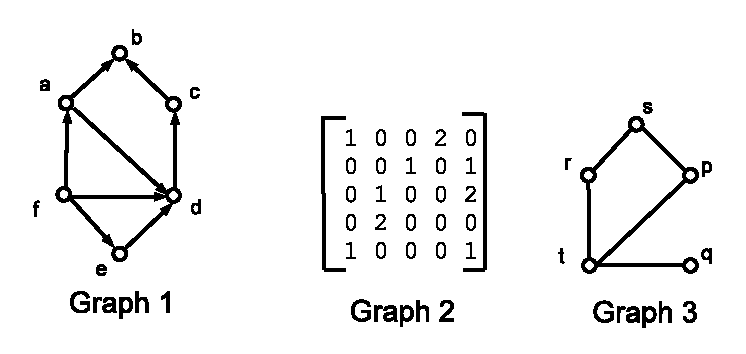
\includegraphics[width=0.6\textwidth]{figs/graph-representation.eps}
\end{center}
\ugquestion{10} Consider Graphs 1-3 above.  Determine the adjacency list for Graph 1. Draw the graph represented by the adjacency matrix for Graph 2 (label the nodes: v, w, x, y, z). Determine the adjacency matrix for Graph 3. 

    \ifprintanswers
        \vspace{-10pt}
    \fi
    \begin{solution}
    \begin{minipage}[t]{0.2\textwidth}
        \begin{tabular}{c|l}
            Node & List \\
            \hline
            a & b, d \\
            b &      \\
            c & b    \\
            d & c    \\
            e & d    \\
            f & a, d, e
        \end{tabular}
    \end{minipage}
    %
    \begin{minipage}[T]{0.3\textwidth}
        \begin{tikzpicture}[scale=0.8]
    \tikzset{VertexStyle/.style = {shape = circle,
                                    color = black,
                                    inner sep=1pt,
                                    minimum size = 8 pt,
                                    font=\scriptsize\sffamily,
                                    draw}}
    %\grEmptyGrid[RA=1.5,RB=1.5]{3}{3}
    \SetGraphUnit{2}
    %\GraphInit[vstyle=Welsh]
    \Vertex[LabelOut,Lpos=-120]{z}
    \NOEA[LabelOut,Lpos=45](z){v}
    \SOEA[LabelOut,Lpos=-90](z){x}
    \EA[LabelOut,Lpos=0](v){y}
    \EA[LabelOut,Lpos=0](x){w}
    
    \tikzset{EdgeStyle/.style = {->}}
    \Edge[style=bend right](v)(y)
    \Edge[style=bend left](v)(y)
    \Edge[style=bend right](y)(w)
    \Edge[style=bend left](y)(w)
    \Edge[style=bend left](x)(w)
    \Edge[style=bend left](w)(x)
    \Edge[style=bend right](w)(z)
    \Edge[style=bend right](x)(z)
    \Edge[style=bend left](x)(z)
    \Edge(z)(v)
    \tikzset{every loop/.style={min distance=10mm,in=-135,out=135,looseness=10}}
    \path[->] (v) edge [loop above] node {} ();
    \path[->] (z) edge [loop left] node {} ();
    % \Loop(o)

\end{tikzpicture}
    \end{minipage}
    %
    \hspace{0.3in}
    \begin{minipage}[T]{0.2\textwidth}
        % $ \begin{bmatrix}
        %   0 & 1 & 1 & 0 & 0 & 0 \\
        %   1 & 0 & 1 & 1 & 0 & 0 \\
        %   1 & 1 & 0 & 1 & 1 & 0 \\
        %   0 & 1 & 1 & 0 & 1 & 1 \\
        %   0 & 0 & 1 & 1 & 0 & 1 \\
        %   0 & 0 & 0 & 1 & 1 & 0 \\
        % \end{bmatrix} $
        node ordering: p, q, r, s, t \\
        $ \begin{bmatrix}
            0 & 0 & 0 & 1 & 1 \\
            0 & 0 & 0 & 0 & 1 \\
            0 & 0 & 0 & 1 & 1 \\
            1 & 0 & 1 & 0 & 0 \\
            1 & 1 & 1 & 0 & 0 \\
        \end{bmatrix} $
    \end{minipage}
    \end{solution}




\gquestion{9}{6}{b-c} Rosen Ch 10.3.58, p. 713.
    \ifprintanswers
        \vspace{-10pt}
    \fi
    \begin{solution}
        (a) 2 $\;\;$ (b) 4 $\;\;$ (c) 11
            \tikzset{mnode/.style = {shape = circle,
                                    color = black,
                                    inner sep=1pt,
                                    minimum size = 4 pt,
                                    font=\scriptsize\sffamily,
                                    draw}}
\begin{tabular}{|c|c||c|c|c|c|}
	\hline
	\multicolumn{2}{|c||}{$n=2$} 
	& \multicolumn{4}{c|}{$n=3$} \\
	\begin{tikzpicture}[mnode/.style = {shape = circle,
                                    color = black,
                                    inner sep=1pt,
                                    minimum size = 4 pt,
                                    font=\scriptsize\sffamily,
                                    draw}]
		\node[mnode] (1) at (0,0) {};
		\node[mnode] (2) at (1,0) {};
	\end{tikzpicture}
	& 
	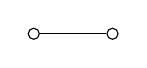
\begin{tikzpicture}[mnode/.style = {shape = circle,
                                    color = black,
                                    inner sep=1pt,
                                    minimum size = 4 pt,
                                    font=\scriptsize\sffamily,
                                    draw}]
		\node[mnode] (1) at (0,0) {};
		\node[mnode] (2) at (1,0) {};
		\path (1) edge (2);
	\end{tikzpicture}
	& 
	\begin{tikzpicture}[mnode/.style = {shape = circle,
                                    color = black,
                                    inner sep=1pt,
                                    minimum size = 4 pt,
                                    font=\scriptsize\sffamily,
                                    draw}]
		\node[mnode] (1) at (0,0) {};
		\node[mnode] (2) at (1,0) {};
		\node[mnode] (3) at (60:1) {};
	\end{tikzpicture}
	& 
	\begin{tikzpicture}[mnode/.style = {shape = circle,
                                    color = black,
                                    inner sep=1pt,
                                    minimum size = 4 pt,
                                    font=\scriptsize\sffamily,
                                    draw}]
		\node[mnode] (1) at (0,0) {};
		\node[mnode] (2) at (1,0) {};
		\node[mnode] (3) at (60:1) {};
		\path (1) edge (2);
	\end{tikzpicture}
	& 
	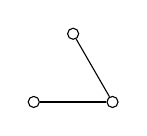
\begin{tikzpicture}[mnode/.style = {shape = circle,
                                    color = black,
                                    inner sep=1pt,
                                    minimum size = 4 pt,
                                    font=\scriptsize\sffamily,
                                    draw}]
		\node[mnode] (1) at (0,0) {};
		\node[mnode] (2) at (1,0) {};
		\node[mnode] (3) at (60:1) {};
		\path (1) edge (2);
		\path (2) edge (3);
	\end{tikzpicture}
	& 
	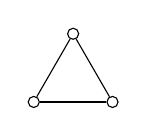
\begin{tikzpicture}[mnode/.style = {shape = circle,
                                    color = black,
                                    inner sep=1pt,
                                    minimum size = 4 pt,
                                    font=\scriptsize\sffamily,
                                    draw}]
		\node[mnode] (1) at (0,0) {};
		\node[mnode] (2) at (1,0) {};
		\node[mnode] (3) at (60:1) {};
		\path (1) edge (2);
		\path (2) edge (3);
		\path (3) edge (1);
	\end{tikzpicture}
	\\
	\hline
\end{tabular}

\begin{tabular}{|c|c|c|c|c|c|c|}
	\hline
	\multicolumn{7}{|c|}{$n=4$} \\
	\begin{tikzpicture}[mnode/.style = {shape = circle,
                                    color = black,
                                    inner sep=1pt,
                                    minimum size = 4 pt,
                                    font=\scriptsize\sffamily,
                                    draw}]
		\node[mnode] (1) at (0,0) {};
		\node[mnode] (2) at (1,0) {};
		\node[mnode] (3) at (1,1) {};
		\node[mnode] (4) at (0,1) {};
	\end{tikzpicture}
	& 
	\begin{tikzpicture}[mnode/.style = {shape = circle,
                                    color = black,
                                    inner sep=1pt,
                                    minimum size = 4 pt,
                                    font=\scriptsize\sffamily,
                                    draw}]
		\node[mnode] (1) at (0,0) {};
		\node[mnode] (2) at (1,0) {};
		\node[mnode] (3) at (1,1) {};
		\node[mnode] (4) at (0,1) {};
		\path (1) edge (2);
	\end{tikzpicture}
	& 
	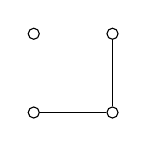
\begin{tikzpicture}[mnode/.style = {shape = circle,
                                    color = black,
                                    inner sep=1pt,
                                    minimum size = 4 pt,
                                    font=\scriptsize\sffamily,
                                    draw}]
		\node[mnode] (1) at (0,0) {};
		\node[mnode] (2) at (1,0) {};
		\node[mnode] (3) at (1,1) {};
		\node[mnode] (4) at (0,1) {};
		\path (1) edge (2);
		\path (2) edge (3);
	\end{tikzpicture}
	& 
	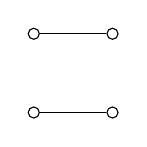
\begin{tikzpicture}[mnode/.style = {shape = circle,
                                    color = black,
                                    inner sep=1pt,
                                    minimum size = 4 pt,
                                    font=\scriptsize\sffamily,
                                    draw}]
		\node[mnode] (1) at (0,0) {};
		\node[mnode] (2) at (1,0) {};
		\node[mnode] (3) at (1,1) {};
		\node[mnode] (4) at (0,1) {};
		\path (1) edge (2);
		\path (3) edge (4);
	\end{tikzpicture}
	& 
	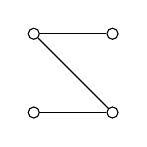
\begin{tikzpicture}[mnode/.style = {shape = circle,
                                    color = black,
                                    inner sep=1pt,
                                    minimum size = 4 pt,
                                    font=\scriptsize\sffamily,
                                    draw}]
		\node[mnode] (1) at (0,0) {};
		\node[mnode] (2) at (1,0) {};
		\node[mnode] (3) at (1,1) {};
		\node[mnode] (4) at (0,1) {};
		\path (1) edge (2);
		\path (2) edge (4);
		\path (4) edge (3);
	\end{tikzpicture}
	&
	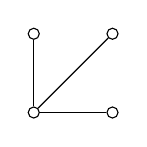
\begin{tikzpicture}[mnode/.style = {shape = circle,
                                    color = black,
                                    inner sep=1pt,
                                    minimum size = 4 pt,
                                    font=\scriptsize\sffamily,
                                    draw}]
		\node[mnode] (1) at (0,0) {};
		\node[mnode] (2) at (1,0) {};
		\node[mnode] (3) at (1,1) {};
		\node[mnode] (4) at (0,1) {};
		\path (1) edge (2);
		\path (1) edge (3);
		\path (1) edge (4);
	\end{tikzpicture}
	& 
	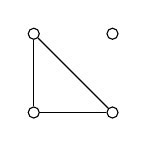
\begin{tikzpicture}[mnode/.style = {shape = circle,
                                    color = black,
                                    inner sep=1pt,
                                    minimum size = 4 pt,
                                    font=\scriptsize\sffamily,
                                    draw}]
		\node[mnode] (1) at (0,0) {};
		\node[mnode] (2) at (1,0) {};
		\node[mnode] (3) at (1,1) {};
		\node[mnode] (4) at (0,1) {};
		\path (1) edge (2);
		\path (1) edge (4);
		\path (2) edge (4);
	\end{tikzpicture} 
	\\
	\hline
	\multicolumn{7}{|c|}{ } \\
	 & 
	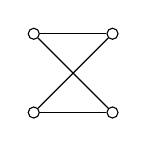
\begin{tikzpicture}[mnode/.style = {shape = circle,
                                    color = black,
                                    inner sep=1pt,
                                    minimum size = 4 pt,
                                    font=\scriptsize\sffamily,
                                    draw}]
		\node[mnode] (1) at (0,0) {};
		\node[mnode] (2) at (1,0) {};
		\node[mnode] (3) at (1,1) {};
		\node[mnode] (4) at (0,1) {};
		\path (1) edge (2);
		\path (3) edge (4);
		\path (1) edge (3);
		\path (2) edge (4);
	\end{tikzpicture}
	& 
	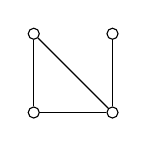
\begin{tikzpicture}[mnode/.style = {shape = circle,
                                    color = black,
                                    inner sep=1pt,
                                    minimum size = 4 pt,
                                    font=\scriptsize\sffamily,
                                    draw}]
		\node[mnode] (1) at (0,0) {};
		\node[mnode] (2) at (1,0) {};
		\node[mnode] (3) at (1,1) {};
		\node[mnode] (4) at (0,1) {};
		\path (1) edge (2);
		\path (1) edge (4);
		\path (2) edge (4);
		\path (2) edge (3);
	\end{tikzpicture}
	& 
	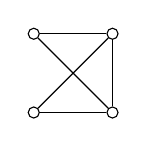
\begin{tikzpicture}[mnode/.style = {shape = circle,
                                    color = black,
                                    inner sep=1pt,
                                    minimum size = 4 pt,
                                    font=\scriptsize\sffamily,
                                    draw}]
		\node[mnode] (1) at (0,0) {};
		\node[mnode] (2) at (1,0) {};
		\node[mnode] (3) at (1,1) {};
		\node[mnode] (4) at (0,1) {};
		\path (1) edge (2);
		\path (3) edge (4);
		\path (1) edge (3);
		\path (2) edge (4);
		\path (2) edge (3);
	\end{tikzpicture}
	& 
	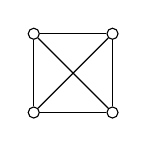
\begin{tikzpicture}[mnode/.style = {shape = circle,
                                    color = black,
                                    inner sep=1pt,
                                    minimum size = 4 pt,
                                    font=\scriptsize\sffamily,
                                    draw}]
		\node[mnode] (1) at (0,0) {};
		\node[mnode] (2) at (1,0) {};
		\node[mnode] (3) at (1,1) {};
		\node[mnode] (4) at (0,1) {};
		\path (1) edge (2);
		\path (3) edge (4);
		\path (1) edge (3);
		\path (2) edge (4);
		\path (2) edge (3);
		\path (1) edge (4);
	\end{tikzpicture}
	& 
	& 
	\\
	\hline
\end{tabular}

    \end{solution}




\ugquestion{3} Rosen Ch 10.3.74(a), p. 713.
    \ifprintanswers
        \vspace{-10pt}
    \fi
    \begin{solution}
        3 graphs, \vspace{-15pt}
\begin{center}
\begin{minipage}[m]{0.2\linewidth}
\vspace{0pt}
\centering
\begin{tikzpicture}
    \tikzset{VertexStyle/.style = {shape = circle,
                                    color = black,
                                    fill = black,
                                    inner sep = 0.5pt,
                                    minimum size = 4pt,
                                    font=\scriptsize\sffamily,
                                    radius=0.1
                                    draw}}
    \SetGraphUnit{1}
    \SetVertexNoLabel
    \Vertex{A}
    \EA(A){B}
\end{tikzpicture}
\end{minipage}
%
\begin{minipage}[m]{0.2\linewidth}
\vspace{0pt}
\centering
\begin{tikzpicture}
    \tikzset{VertexStyle/.style = {shape = circle,
                                    color = black,
                                    fill = black,
                                    inner sep = 0.5pt,
                                    minimum size = 4pt,
                                    font=\scriptsize\sffamily,
                                    radius=0.1
                                    draw}}
    %\grEmptyGrid[RA=1.5,RB=1.5]{3}{3}
    \SetGraphUnit{1}
    \SetVertexNoLabel
    %\GraphInit[vstyle=Hasse]

    \Vertex{A}
    \EA(A){B}
    \Edge[style={->,bend right}](A)(B)
    \Edge[style={->,bend right}](B)(A)
\end{tikzpicture}
\end{minipage}
%
\begin{minipage}[m]{0.2\linewidth}
\vspace{0pt}
\centering
\begin{tikzpicture}
    \tikzset{VertexStyle/.style = {shape = circle,
                                    color = black,
                                    fill = black,
                                    inner sep = 0.5pt,
                                    minimum size = 4pt,
                                    font=\scriptsize\sffamily,
                                    radius=0.1
                                    draw}}
    %\grEmptyGrid[RA=1.5,RB=1.5]{3}{3}
    \SetGraphUnit{1}
    \SetVertexNoLabel
    %\GraphInit[vstyle=Hasse]

    \Vertex{A}
    \EA(A){B}
    \Edge[style={->}](A)(B)
\end{tikzpicture}
\end{minipage}
%
\end{center}
    \end{solution}



\gquestion{6}{2}{b} Rosen Ch 10.4.2a,b,c, p. 724.
   \ifprintanswers
        \vspace{-15pt}
   \fi
    \begin{solution}
    \begin{tabular}{lcccc}
        Vertices & Path? & Simple? & Circuit? & Length? \\
        \hline
        a) $a,b,e,c,b$     & Y & Y & N & 4 \\
        b) $a,d,a,d,a$     & Y & N & Y & 4 \\
        c) $a,d,b,e,a$     & N & -- & -- & -- \\
        \hline
    \end{tabular}
    \end{solution}



\gquestion{6}{2}{a} Rosen Ch 10.4.12, p. 725.
   \ifprintanswers
        \vspace{-15pt}
   \fi
    \begin{solution}
    % \begin{parts}
    \begin{enumerate}[label=(\alph*), topsep=0pt, itemsep=0pt, parsep=0pt]
        \item not strongly connected, weakly connected.
        \item  strongly connected and weakly connected.
        \item  neither strongly nor weakly connected.
    % \end{parts}
    \end{enumerate}
    \end{solution}



\ugquestion{6} Rosen Ch 10.4.14(a,b), p. 725
    \ifprintanswers
        \vspace{-15pt}
    \fi
    \begin{solution}
    % \begin{parts}
    \begin{enumerate}[label=(\alph*), topsep=0pt, itemsep=0pt, parsep=0pt]
        \item  $\{a,b,e\}, \{ c\}, \{d\} $  \hfill
        \item  $ \{a\}, \{b\}, \{c,d,e\}, \{f\} $ \hfill
        \item  $ \{a,b,c,d,f,g,h,i\}, \{e\} $
    % \end{parts}
    \end{enumerate}
    \end{solution}



\ugquestion{4} Determine the cut vertices and edges for the graphs of Rosen Ch 10.4, Exercise 31 \& 32, p. 726.
    \ifprintanswers
        \vspace{-10pt}
    \fi
    \begin{solution}
        For the graph of Ex. 31, the cut vertex is $c$ and there are no cut edges. 

        For the graph of Ex. 32, the cut vertices are $c$ and $d$, the cut edge is $\{c, d\}$.
    \end{solution} 
    




\gquestion{14}{6}{b-d}  For each graph, determine whether it has an Euler circuit and an Euler path.  If a circuit or path exists, construct an example.
\begin{enumerate}[label=(\alph*), topsep=0pt, itemsep=0pt, parsep=0pt]
    \item Rosen Ch 10.1.4, p.683
    \item Rosen Ch 10.2.22, p. 700
    \item Rosen Ch 10.2.23, p. 700
    \item Rosen Ch 10.2.24, p. 700

    For the directed graphs, read the conditions expressed in Rosen Ch 10.5.16-17.  
    \item Rosen Ch 10.1.7, p. 683
    \item Rosen Ch 10.5.18, p. 740
    \item Rosen Ch 10.5.20, p. 740

    % \item Rosen Ch 10.2, Figure 8, graph $G$, p. 656
    % \item Rosen Ch 10.2.22, p. 700
    % \item Rosen Ch 10.2.24, p. 700
    % % \item Rosen Ch 10.4, Exercise 31, p. 691
    % % \item Rosen Ch 10.4, Exercise 20, graph $H$, p. 690
    % \item Rosen Ch 10.4.14(b), p. 725
    % \item Rosen Ch 10.5, Exercise 35, p. 705
\end{enumerate}

\ifprintanswers 
\else
Present answers as table: 

\begin{tabular}{|c||l|l||l|l|}
    \hline 
          & Euler & Euler &  & \\
          & Circuit? & Path? & Example Circuit & Example Path \\
    \hline 
        (a) & Yes/No & Yes/No & a, b, c, \ldots \hspace*{0.8in}  & --- \hspace*{1in} \\
    \hline 
        (b) & & & & \\
    \hline 
\end{tabular}
\fi

    \ifprintanswers
        \vspace{-10pt}
   \fi
    \begin{solution}
        \begin{tabular}{|c|ll|ll|}
        \hline 
              & Euler & Euler &  & \\
              & Circuit? & Path? & Example Circuit & Example Path \\
        \hline 
            (a) & No & Yes & ---  & a, b, d, b, d, c, a, b \\
        \hline 
            (b) & No & Yes & ---  & a, b, c, e, a, d, c \\
        \hline 
            (c) & No & Yes & ---  & a, b, c, d, a, e, c, f, b \\
        \hline 
            (d) & Yes & Yes & a, c, b, f, d, c, e, f, a & a, c, b, f, d, c, e, f, a \\
        \hline
            (e) & No  & No  & --- &  --- \\
        \hline 
            (f) & No & Yes  & --- & a,b,d,b,c,d,c,a,d \\
        \hline 
            (g) & Yes & Yes & a,d,b,d,e,b,e,c,b,a & a,d,b,d,e,b,e,c,b,a \\
        \hline 
        \end{tabular} 

    % Explaination:
    % \begin{enumerate}[label=(\alph*), topsep=0pt, itemsep=0pt, parsep=0pt]
    %     \item The graph has two vertices $a$ and $b$ of odd degree, therefore, no Euler circuit, but it does have an Euler path. 
    %     \item No Euler circuit, the degree of vertex $a$ and $c$ are odd. It does have an Euler path.
    %     \item No Euler circuit, the degree of vertex $a$ and $b$ are odd. It does have an Euler path.
    %     \item Euler circuit: an example $a, c, b, f, d, c, e, f, a$; other circuits exist.  Each Euler circuit is also a path.
    %     \item No Euler circuit and no Euler path.
    %     \item 
    % \end{enumerate}

    % \begin{enumerate}[label=(\alph*), topsep=0pt, itemsep=0pt, parsep=0pt]
        % \item No Euler path and no Euler circuit; the graph has more than two vertices of an odd degree
        % \item No Euler circuit, the degree of vertex $a$ and $c$ are odd. There are Euler paths: an example $a, b, c, d, a, e, c$
        % \item Euler circuit: an example $a, c, b, f, d, c, e, f, a$; other circuits exist.  Each Euler circuit is also a path.
        % % \item Euler circuit: two examples $a, b, c, d, e, f, c, a$ or $a, b, c, f, e, d, c, a$; other circuits exist.  Each Euler circuit is also a path. 
        % % \item No Euler path and no Euler circuit exists (the graph has more than two vertices of an odd degree).
        % \item No Euler circuit and no Euler path.
        % \item No Euler circuits, the degree of vertex $b$ and $c$ are odd. 
        %     There are a Euler paths.  One such path is: $b, e, c, a, b, d, c$.
    % \end{enumerate}
    \end{solution}



\gquestion{6}{6}{a-c} Rosen Ch 10.5.26(a,b,c), p. 740.
    \ifprintanswers
        \vspace{-10pt}
    \fi
    \begin{solution}
    \begin{enumerate}[label=(\alph*), topsep=0pt, itemsep=0pt, parsep=0pt]
        \item There is a Euler circuit if $n$ is odd and $n>1$
        \item For all $n\geq3$, $C_n$ has a Euler circuit
        \item No wheel graph has a Euler circuit
    \end{enumerate}
    \end{solution}



\gquestion{10}{6}{a-c} For each graph, determine whether it has a Hamilton circuit and a Hamilton path.  If a circuit or path exists, construct an example.
\begin{enumerate}[label=(\alph*), topsep=0pt, itemsep=0pt, parsep=0pt]
    % \item Rosen Ch 10.2, Exercise 25, p. 666
    \item Rosen Ch 10.3, Figure 1, p. 668
    \item Rosen Ch 10.3, Figure 10, graph $H$, p. 673
    % \item Rosen Ch 10.4, Exercise 20, graph $G$, p. 690
    \item Rosen Ch 10.4.33, p. 726
    \item Rosen, Ch 10.4.14(b), p. 725
    \item Rosen, Ch 10.5.6, p. 739
\end{enumerate}

Present results in a table like Problem 11. 

    \ifprintanswers
        \vspace{-10pt}
   \fi
    \begin{solution}
        \begin{tabular}{|c|ll|ll|}
        \hline 
              & Hamilton & Hamilton &  & \\
              & Circuit? & Path? & Example Circuit & Example Path \\
        \hline 
            (a) & No & Yes & ---  & $b, a, c, d, e$ \\
        \hline 
            (b) & Yes & Yes & $s, w, x, y, z, v, u, t, s$ & $s, w, x, y, z, v, u, t$ \\
        \hline 
            (c) & No & No & ---  & --- \\
        \hline 
            (d) & No & Yes & --- & $c, d, e, b, a, f$ \\
        \hline
            (e) & No  & Yes  & --- &  $e, f, d, g, i, h, a, b, c$. \\
        \hline 
        \end{tabular} 


    % \begin{enumerate}[label=(\alph*), topsep=0pt, itemsep=0pt, parsep=0pt]
    %     % \item Hamilton circuit: one such circuit is $a, b, e, d, c, f, a$; Each Hamilton circuit is also a path
    %     \item No Hamilton circuits.  An example Hamilton path is $b, a, c, d, e$
    %     \item Hamilton circuit: an example $s, w, x, y, z, v, u, t, s$. Each Hamilton circuit is also a path
    %     % \item Hamilton circuit: $v_1, v_4, v_3, v_2, v_6, v_7, v_8, v_5, v_1$ \\ 
    %     % A  Hamilton path: $v_1, v_4, v_3, v_2, v_6, v_7, v_8, v_5$
    %     \item No Hamilton path and no Hamilton circuit
    %     \item No Hamilton circuits. An example Hamilton path is $c, d, e, b, a, f$
    %     \item No Hamilton circuits.  Notice, vertex $d$ would need to be visited twice to include vertices $e$ and $f$ in the circuit.  
    %     There is a Hamilton path.  One such path is: $e, f, d, g, i, h, a, b, c$.
    % \end{enumerate}
    \end{solution}




\gquestion{6}{4}{b,c} Determine whether each graph is planar, if it is give a planar representation.
\begin{enumerate}[label=(\alph*), topsep=0pt,itemsep=0pt,parsep=0pt]
    \item Rosen Ch 10.7.2, p. 760 
    \item Rosen Ch 10.7.6, p. 760
    \item Rosen Ch 10.7.8, p. 760
\end{enumerate}
    \ifprintanswers
        \vspace{-10pt}
    \fi
    \begin{solution}
    % \begin{enumerate}[label=(\alph*), topsep=0pt,itemsep=0pt,parsep=0pt]
    %   \item Planar
    %   \item Planar
    %   \item Not planar
    % \end{enumerate}
    \begin{center}
    \begin{tabular}[t]{ccp{3in}}
        (a) Planar & (b) Planar &  (c) Not Planar \\
        \begin{minipage}[b][0.4in][t]{0.9in} %[minipage place][height][content align]{width}
        \begin{tikzpicture}[scale=0.55]
            %\GraphInit[vstyle=Welsh]
            \tikzset{VertexStyle/.style = {shape = circle,
                                            %ball color = orange,
                                            text = black,
                                            inner sep = 1pt,
                                            outer sep = 0pt,
                                            minimum size = 4 pt,
                                            draw}}
            \SetGraphUnit{3}
            \Vertex[x=0,y=0,Lpos=180,LabelOut]{a}
            \Vertex[x=2,y=0,Lpos=0,LabelOut]{b}
            \Vertex[x=0,y=2,Lpos=180,LabelOut]{c}
            \Vertex[x=2,y=2,Lpos=0,LabelOut]{d}
            \Vertex[x=1,y=1,Lpos=0,LabelOut]{e}
            \tikzset{EdgeStyle/.style = {-,line width=0.75pt}}
            \Edge(a)(b)
            \Edge(b)(d)
            \Edge(a)(c)
            \Edge(c)(d)
            \Edge(d)(e)
            \Edge(a)(e)
        \end{tikzpicture}
        \end{minipage}
        &  
        \hspace*{0.5in}
        \begin{minipage}[b][0.4in][t]{1.1in}
        \begin{tikzpicture}[scale=0.55]
            %\GraphInit[vstyle=Welsh]
            \tikzset{VertexStyle/.style = {shape = circle,
                                            %ball color = orange,
                                            text = black,
                                            inner sep = 1pt,
                                            outer sep = 0pt,
                                            minimum size = 4 pt,
                                            draw}}
            \SetGraphUnit{3}
            \Vertex[x=0,y=0,Lpos=225,LabelOut]{e}
            \Vertex[x=0,y=2,Lpos=135,LabelOut]{b}
            \Vertex[x=2,y=0,Lpos=-45,LabelOut]{c}
            \Vertex[x=2,y=2,Lpos=45,LabelOut]{d}
            \Vertex[x=4,y=0,Lpos=-45,LabelOut]{f}
            \Vertex[x=4,y=2,Lpos=45,LabelOut]{a}
            \tikzset{EdgeStyle/.style = {-,line width=0.75pt}}
            \Edge(a)(f)
            \Edge(a)(d)
            \Edge(f)(c)
            \Edge(c)(d)
            \Edge(c)(e)
            \Edge(b)(d)
            \Edge(b)(e)
        \end{tikzpicture}
        \end{minipage}
        \hspace*{0.5in}
        & 
        The graph contains a subgraph homeomorphic to $K_{3,3}$ therefore it can not be planer.  In fact, it has a subgraph of directly $K_{3,3}$ with vertices $\{a, c, e\}$ and $\{ b, d, f\}$
    \end{tabular}
    \end{center}
    \end{solution}



\gquestion{6}{3}{c} For each graph, determine the chromatic number.
\begin{enumerate}[label=(\alph*), topsep=0pt,itemsep=0pt,parsep=0pt]
    \item Rosen Ch 10.2.24, p. 700
    \item Rosen Ch 10.3.2, p. 710
    \item Rosen Ch 10.7.24, p. 761  % s12 - hw 10, # 22
\end{enumerate}
    \ifprintanswers
        \vspace{-10pt}
    \fi
    \begin{solution}
    \begin{enumerate}[label=(\alph*), topsep=0pt,itemsep=0pt,parsep=0pt]
        \item 2 colors
        \item 3 colors
        \item 4 colors, one coloring shown below
    \end{enumerate}
    Exercise 24, p. 726
    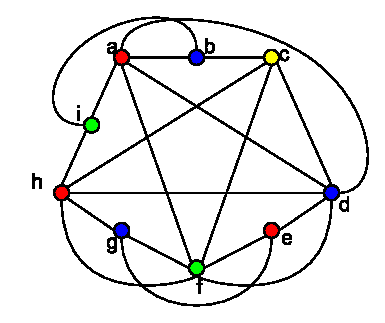
\includegraphics[width=1.8in]{figs/hw10-p22}
    \end{solution}





\section*{Bonus}


% \bonusquestion[2] List all the equivalence relations on the set $\{a, b, c\}$.  (Describe the relation be describing the partition on the set).
%     \ifprintanswers
%         \vspace{-10pt}
%     \fi
%     \begin{solution}
%     There are five such relations
%     \[ \{ \{a\}, \{b\}, \{c\} \}; \{ \{a, b\}, \{c\} \}; \{ \{a, c\}, \{b\} \}; 
%         \{ \{b, c\}, \{a\} \};  \{ \{a, b, c\} \} \]
%     \end{solution}


\bonusquestion[1] Rosen Ch 10.3.48, p. 712
    \ifprintanswers
        \vspace{-10pt}
    \fi
    \begin{solution}
        The two graphs are not isomorphic.  To see this, consider the complement of both graphs.  The complement of the graph on the left consists of two 4-cycles.  The complement of the graph on the right is an 8-cycle.  The complements are not isomorphic, therefore the original graphs are not isomorphic.
    \end{solution}


\bonusquestion[1] Rosen Ch 10.5.28(a), p. 740.
    \ifprintanswers
        \vspace{-10pt}
    \fi
    \begin{solution}
        The graph has a Euler circuit if and only if both positive integers $m$ and $n$ are even.
    \end{solution}



\bonusquestion[3] The \textbf{complementary graph} $G$ is describe in Rosen Ch 10.2.61, p. 702. A graph $G$ is called \textbf{self-complementary} if it is isomorphic to $G$.
    \begin{parts}
        \part Give an example of a self-complementary graph with $|V| = 4$. 
        \part Give an example of a self-complementary graph with $|V| = 5$.
    \end{parts}
    \ifprintanswers
        \vspace{-10pt}
    \fi
    \begin{solution}
        % \input{bp1.tex}
        (a) 
\includegraphics[width=1in]{figs/hw12-bp1a.pdf} \hspace{0.25in} (b) 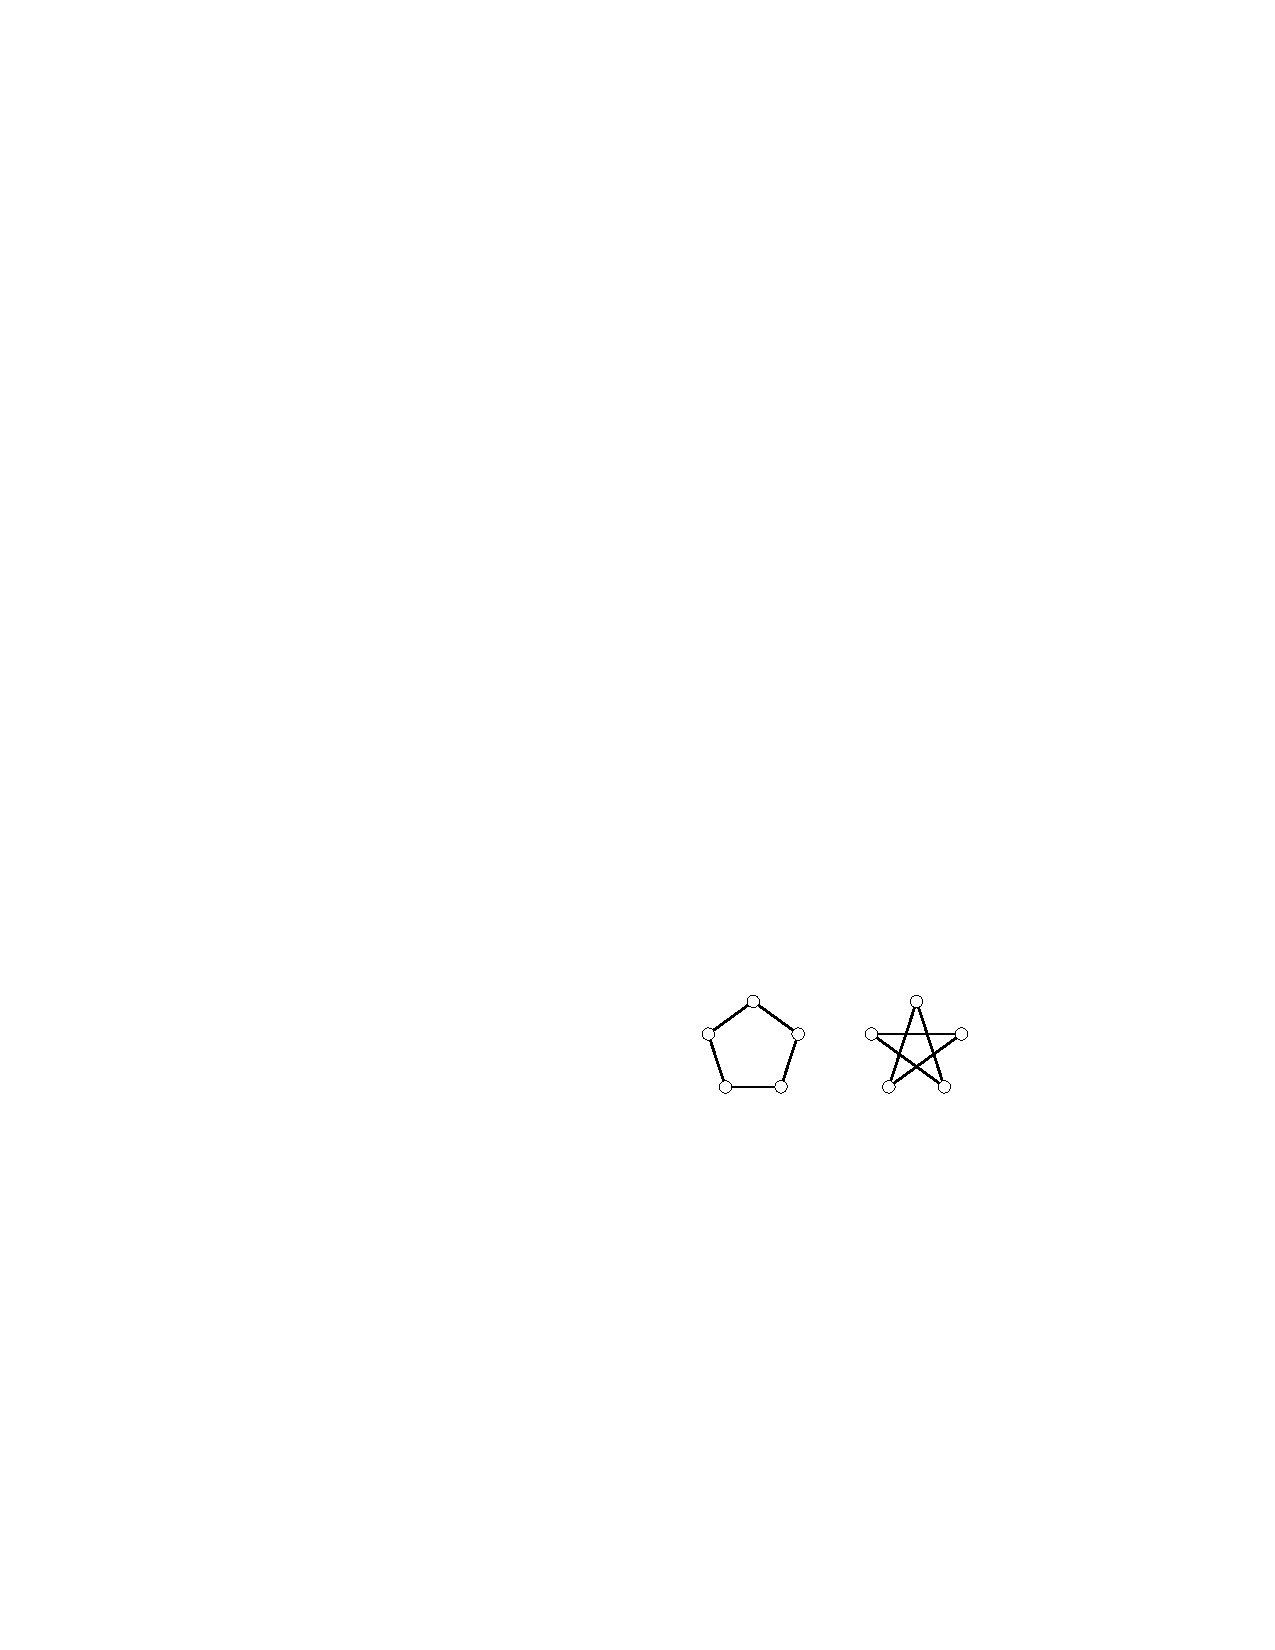
\includegraphics[width=1in]{figs/hw12-bp1b.pdf}
    \end{solution}




\bonusquestion[10]  Consider the set of all non-isomorphic simple undirected graphs (but do allow self-loops) of 3 vertices.  % f09 - hw10, #30 cont.

    \begin{minipage}[T]{0.55\textwidth}
    \begin{enumerate}[label=(\alph*),topsep=1pt,parsep=1pt,itemsep=0pt]
        \item Draw all such graphs. 
        \item  How many are connected? \ifprintanswers \underline{10} \fi
        % \item  How many are complete?  \ifprintanswers \underline{1} \fi
        \item  How many are bipartite? \ifprintanswers \underline{3} \fi
        % \item  How many are complete bipartite? \ifprintanswers \underline{0} \fi
        \item  How many have a Euler circuit? \ifprintanswers \underline{6} \fi
        \item  How many have a Hamiltonian circuit? \ifprintanswers \underline{4} \fi
        \item  How many have a Euler path? \ifprintanswers \underline{15} \fi
        \item  How many have a Hamiltonian path? \ifprintanswers \underline{10} \fi
        \item  How many are planar? \ifprintanswers \underline{20} \fi
    \end{enumerate}
    \end{minipage}
    % \begin{minipage}[T]{2.4in}
    %   % \begin{solution}
    %   % $\chi = 4$, a coloring is: 
        
 %  %       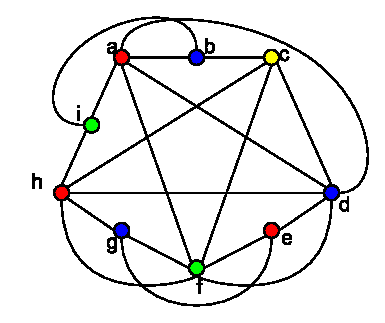
\epsfig{file=figs/hw10-p22.eps,width=1.9in}
 %  %       \end{solution}
 %      \end{minipage}
    \ifprintanswers
        \vspace{-5pt}
    \fi
    \begin{solution}Consider the set of graphs:

        \scriptsize
\begin{minipage}[t]{0.2\linewidth}
\begin{center}
\begin{tikzpicture}[scale=0.45]
    \tikzset{VertexStyle/.style = {shape = circle,
                                    color = black,
                                    fill = black,
                                    inner sep = 1pt,
                                    minimum size = 4pt,
                                    font=\scriptsize\sffamily,
                                    draw}}
    \SetGraphUnit{1}
    \SetVertexNoLabel
    \Vertex{a}
    \Vertex[x=2,y=0]{b}
    \Vertex[x=1,y=1.5]{c}
\end{tikzpicture}
\end{center}
\end{minipage}
\begin{minipage}[t]{0.2\linewidth}
\begin{center}
\begin{tikzpicture}[scale=0.45]
    \tikzset{VertexStyle/.style = {shape = circle,
                                    color = black,
                                    fill = black,
                                    inner sep = 1pt,
                                    minimum size = 4pt,
                                    font=\scriptsize\sffamily,
                                    draw}}
    \SetGraphUnit{1}
    \SetVertexNoLabel
    \Vertex{a}
    \Vertex[x=2,y=0]{b}
    \Vertex[x=1,y=1.5]{c}
    \Edge(a)(c)
\end{tikzpicture}
\end{center}
\end{minipage}
\begin{minipage}[t]{0.2\linewidth}
\begin{center}
\begin{tikzpicture}[scale=0.45]
    \tikzset{VertexStyle/.style = {shape = circle,
                                    color = black,
                                    fill = black,
                                    inner sep = 1pt,
                                    minimum size = 4pt,
                                    font=\scriptsize\sffamily,
                                    draw}}
    \SetGraphUnit{1}
    \SetVertexNoLabel
    \Vertex{a}
    \Vertex[x=2,y=0]{b}
    \Vertex[x=1,y=1.5]{c}
    \Edge(a)(c)
    \Edge(a)(b)
\end{tikzpicture}
\end{center}
\end{minipage}
\begin{minipage}[t]{0.2\linewidth}
\begin{center}
\begin{tikzpicture}[scale=0.45]
    \tikzset{VertexStyle/.style = {shape = circle,
                                    color = black,
                                    fill = black,
                                    inner sep = 1pt,
                                    minimum size = 4pt,
                                    font=\scriptsize\sffamily,
                                    draw}}
    \SetGraphUnit{1}
    \SetVertexNoLabel
    \Vertex{a}
    \Vertex[x=2,y=0]{b}
    \Vertex[x=1,y=1.5]{c}
    \Edge(a)(c)
    \Edge(a)(b)
    \Edge(b)(c)
\end{tikzpicture}
\end{center}
\end{minipage}



\vspace{0.05in}
\hrule
\vspace{0.05in}



\begin{minipage}[t]{0.15\linewidth}
\begin{center}
\begin{tikzpicture}[scale=0.45]
    \tikzset{VertexStyle/.style = {shape = circle,
                                    color = black,
                                    fill = black,
                                    inner sep = 1pt,
                                    minimum size = 4pt,
                                    font=\scriptsize\sffamily,
                                    draw}}
    \SetGraphUnit{1}
    \SetVertexNoLabel
    \Vertex{a}
    \Vertex[x=2,y=0]{b}
    \Vertex[x=1,y=1.5]{c}
    \Loop[dist=1cm,dir=WE,style={-}](a)
\end{tikzpicture}
\end{center}
\end{minipage}
\begin{minipage}[t]{0.15\linewidth}
\begin{center}
\begin{tikzpicture}[scale=0.45]
    \tikzset{VertexStyle/.style = {shape = circle,
                                    color = black,
                                    fill = black,
                                    inner sep = 1pt,
                                    minimum size = 4pt,
                                    font=\scriptsize\sffamily,
                                    draw}}
    \SetGraphUnit{1}
    \SetVertexNoLabel
    \Vertex{a}
    \Vertex[x=2,y=0]{b}
    \Vertex[x=1,y=1.5]{c}
    \Edge(a)(c)
    \Loop[dist=1cm,dir=WE,style={-}](a)
\end{tikzpicture}
\end{center}
\end{minipage}
\begin{minipage}[t]{0.15\linewidth}
\begin{center}
\begin{tikzpicture}[scale=0.45]
    \tikzset{VertexStyle/.style = {shape = circle,
                                    color = black,
                                    fill = black,
                                    inner sep = 1pt,
                                    minimum size = 4pt,
                                    font=\scriptsize\sffamily,
                                    draw}}
    \SetGraphUnit{1}
    \SetVertexNoLabel
    \Vertex{a}
    \Vertex[x=2,y=0]{b}
    \Vertex[x=1,y=1.5]{c}
    \Edge(b)(c)
    \Loop[dist=1cm,dir=WE,style={-}](a)
\end{tikzpicture}
\end{center}
\end{minipage}
\begin{minipage}[t]{0.15\linewidth}
\begin{center}
\begin{tikzpicture}[scale=0.45]
    \tikzset{VertexStyle/.style = {shape = circle,
                                    color = black,
                                    fill = black,
                                    inner sep = 1pt,
                                    minimum size = 4pt,
                                    font=\scriptsize\sffamily,
                                    draw}}
    \SetGraphUnit{1}
    \SetVertexNoLabel
    \Vertex{a}
    \Vertex[x=2,y=0]{b}
    \Vertex[x=1,y=1.5]{c}
    \Edge(a)(c)
    \Edge(a)(b)
    \Loop[dist=1cm,dir=WE,style={-}](a)
\end{tikzpicture}
\end{center}
\end{minipage}
\begin{minipage}[t]{0.15\linewidth}
\begin{center}
\begin{tikzpicture}[scale=0.45]
    \tikzset{VertexStyle/.style = {shape = circle,
                                    color = black,
                                    fill = black,
                                    inner sep = 1pt,
                                    minimum size = 4pt,
                                    font=\scriptsize\sffamily,
                                    draw}}
    \SetGraphUnit{1}
    \SetVertexNoLabel
    \Vertex{a}
    \Vertex[x=2,y=0]{b}
    \Vertex[x=1,y=1.5]{c}
    \Edge(b)(c)
    \Edge(a)(c)
    \Loop[dist=1cm,dir=WE,style={-}](a)
\end{tikzpicture}
\end{center}
\end{minipage}
\begin{minipage}[t]{0.15\linewidth}
\begin{center}
\begin{tikzpicture}[scale=0.45]
    \tikzset{VertexStyle/.style = {shape = circle,
                                    color = black,
                                    fill = black,
                                    inner sep = 1pt,
                                    minimum size = 4pt,
                                    font=\scriptsize\sffamily,
                                    draw}}
    \SetGraphUnit{1}
    \SetVertexNoLabel
    \Vertex{a}
    \Vertex[x=2,y=0]{b}
    \Vertex[x=1,y=1.5]{c}
    \Edge(a)(b)
    \Edge(a)(c)
    \Edge(b)(c)
    \Loop[dist=1cm,dir=WE,style={-}](a)
\end{tikzpicture}
\end{center}
\end{minipage}



\vspace{0.05in}
\hrule
\vspace{0.05in}



\begin{minipage}[t]{0.15\linewidth}
\begin{center}
\begin{tikzpicture}[scale=0.45]
    \tikzset{VertexStyle/.style = {shape = circle,
                                    color = black,
                                    fill = black,
                                    inner sep = 1pt,
                                    minimum size = 4pt,
                                    font=\scriptsize\sffamily,
                                    draw}}
    \SetGraphUnit{1}
    \SetVertexNoLabel
    \Vertex{a}
    \Vertex[x=2,y=0]{b}
    \Vertex[x=1,y=1.5]{c}
    \Loop[dist=1cm,dir=WE,style={-}](a)
    \Loop[dist=1cm,dir=EA,style={-}](b)
\end{tikzpicture}
\end{center}
\end{minipage}
\begin{minipage}[t]{0.15\linewidth}
\begin{center}
\begin{tikzpicture}[scale=0.45]
    \tikzset{VertexStyle/.style = {shape = circle,
                                    color = black,
                                    fill = black,
                                    inner sep = 1pt,
                                    minimum size = 4pt,
                                    font=\scriptsize\sffamily,
                                    draw}}
    \SetGraphUnit{1}
    \SetVertexNoLabel
    \Vertex{a}
    \Vertex[x=2,y=0]{b}
    \Vertex[x=1,y=1.5]{c}
    \Edge(a)(c)
    \Loop[dist=1cm,dir=WE,style={-}](a)
    \Loop[dist=1cm,dir=EA,style={-}](b)
\end{tikzpicture}
\end{center}
\end{minipage}
\begin{minipage}[t]{0.15\linewidth}
\begin{center}
\begin{tikzpicture}[scale=0.45]
    \tikzset{VertexStyle/.style = {shape = circle,
                                    color = black,
                                    fill = black,
                                    inner sep = 1pt,
                                    minimum size = 4pt,
                                    font=\scriptsize\sffamily,
                                    draw}}
    \SetGraphUnit{1}
    \SetVertexNoLabel
    \Vertex{a}
    \Vertex[x=2,y=0]{b}
    \Vertex[x=1,y=1.5]{c}
    \Edge(a)(b)
    \Loop[dist=1cm,dir=WE,style={-}](a)
    \Loop[dist=1cm,dir=EA,style={-}](b)
\end{tikzpicture}
\end{center}
\end{minipage}
\begin{minipage}[t]{0.15\linewidth}
\begin{center}
\begin{tikzpicture}[scale=0.45]
    \tikzset{VertexStyle/.style = {shape = circle,
                                    color = black,
                                    fill = black,
                                    inner sep = 1pt,
                                    minimum size = 4pt,
                                    font=\scriptsize\sffamily,
                                    draw}}
    \SetGraphUnit{1}
    \SetVertexNoLabel
    \Vertex{a}
    \Vertex[x=2,y=0]{b}
    \Vertex[x=1,y=1.5]{c}
    \Edge(a)(c)
    \Edge(a)(b)
    \Loop[dist=1cm,dir=WE,style={-}](a)
    \Loop[dist=1cm,dir=EA,style={-}](b)
\end{tikzpicture}
\end{center}
\end{minipage}
\begin{minipage}[t]{0.15\linewidth}
\begin{center}
\begin{tikzpicture}[scale=0.45]
    \tikzset{VertexStyle/.style = {shape = circle,
                                    color = black,
                                    fill = black,
                                    inner sep = 1pt,
                                    minimum size = 4pt,
                                    font=\scriptsize\sffamily,
                                    draw}}
    \SetGraphUnit{1}
    \SetVertexNoLabel
    \Vertex{a}
    \Vertex[x=2,y=0]{b}
    \Vertex[x=1,y=1.5]{c}
    \Edge(a)(c)
    \Edge(b)(c)
    \Loop[dist=1cm,dir=WE,style={-}](a)
    \Loop[dist=1cm,dir=EA,style={-}](b)
\end{tikzpicture}
\end{center}
\end{minipage}
\begin{minipage}[t]{0.15\linewidth}
\begin{center}
\begin{tikzpicture}[scale=0.45]
    \tikzset{VertexStyle/.style = {shape = circle,
                                    color = black,
                                    fill = black,
                                    inner sep = 1pt,
                                    minimum size = 4pt,
                                    font=\scriptsize\sffamily,
                                    draw}}
    \SetGraphUnit{1}
    \SetVertexNoLabel
    \Vertex{a}
    \Vertex[x=2,y=0]{b}
    \Vertex[x=1,y=1.5]{c}
    \Edge(a)(b)
    \Edge(a)(c)
    \Edge(b)(c)
    \Loop[dist=1cm,dir=WE,style={-}](a)
    \Loop[dist=1cm,dir=EA,style={-}](b)
\end{tikzpicture}
\end{center}
\end{minipage}


\vspace{0.05in}
\hrule
\vspace{0.05in}


\begin{minipage}[t]{0.2\linewidth}
\begin{center}
\begin{tikzpicture}[scale=0.45]
    \clip (-1,-1) rectangle (3, 2.5);
    \tikzset{VertexStyle/.style = {shape = circle,
                                    color = black,
                                    fill = black,
                                    inner sep = 1pt,
                                    minimum size = 4pt,
                                    font=\scriptsize\sffamily,
                                    draw}}
    \SetGraphUnit{1}
    \SetVertexNoLabel
    \Vertex{a}
    \Vertex[x=2,y=0]{b}
    \Vertex[x=1,y=1.5]{c}
    \Loop[dist=1cm,dir=WE,style={-}](a)
    \Loop[dist=1cm,dir=EA,style={-}](b)
    \Loop[dist=1cm,dir=NO,style={-}](c)
\end{tikzpicture}
\end{center}
\end{minipage}
\begin{minipage}[t]{0.2\linewidth}
\begin{center}
\begin{tikzpicture}[scale=0.45]
    \clip (-1,-1) rectangle (3, 2.5);
    \tikzset{VertexStyle/.style = {shape = circle,
                                    color = black,
                                    fill = black,
                                    inner sep = 1pt,
                                    minimum size = 4pt,
                                    font=\scriptsize\sffamily,
                                    draw}}
    \SetGraphUnit{1}
    \SetVertexNoLabel
    \Vertex{a}
    \Vertex[x=2,y=0]{b}
    \Vertex[x=1,y=1.5]{c}
    \Edge(a)(c)
    \Loop[dist=1cm,dir=WE,style={-}](a)
    \Loop[dist=1cm,dir=EA,style={-}](b)
    \Loop[dist=1cm,dir=NO,style={-}](c)
\end{tikzpicture}
\end{center}
\end{minipage}
\begin{minipage}[t]{0.2\linewidth}
\begin{center}
\begin{tikzpicture}[scale=0.45]
    \clip (-1,-1) rectangle (3, 2.5);
    \tikzset{VertexStyle/.style = {shape = circle,
                                    color = black,
                                    fill = black,
                                    inner sep = 1pt,
                                    minimum size = 4pt,
                                    font=\scriptsize\sffamily,
                                    draw}}
    \SetGraphUnit{1}
    \SetVertexNoLabel
    \Vertex{a}
    \Vertex[x=2,y=0]{b}
    \Vertex[x=1,y=1.5]{c}
    \Edge(a)(c)
    \Edge(a)(b)
    \Loop[dist=1cm,dir=WE,style={-}](a)
    \Loop[dist=1cm,dir=EA,style={-}](b)
    \Loop[dist=1cm,dir=NO,style={-}](c)
\end{tikzpicture}
\end{center}
\end{minipage}
\begin{minipage}[t]{0.2\linewidth}
\begin{center}
\begin{tikzpicture}[scale=0.45]
    \clip (-1,-1) rectangle (3, 2.5);
    \tikzset{VertexStyle/.style = {shape = circle,
                                    color = black,
                                    fill = black,
                                    inner sep = 1pt,
                                    minimum size = 4pt,
                                    font=\scriptsize\sffamily,
                                    draw}}
    \SetGraphUnit{1}
    \SetVertexNoLabel
    \Vertex{a}
    \Vertex[x=2,y=0]{b}
    \Vertex[x=1,y=1.5]{c}
    \Edge(a)(b)
    \Edge(a)(c)
    \Edge(b)(c)
    \Loop[dist=1cm,dir=WE,style={-}](a)
    \Loop[dist=1cm,dir=EA,style={-}](b)
    \Loop[dist=1cm,dir=NO,style={-}](c)
\end{tikzpicture}
\end{center}
\end{minipage} 


    \end{solution}


\end{questions}

\end{document}
